\documentclass[tikz, border=1mm]{standalone}
\usetikzlibrary{arrows.meta, decorations.pathreplacing}

\begin{document}
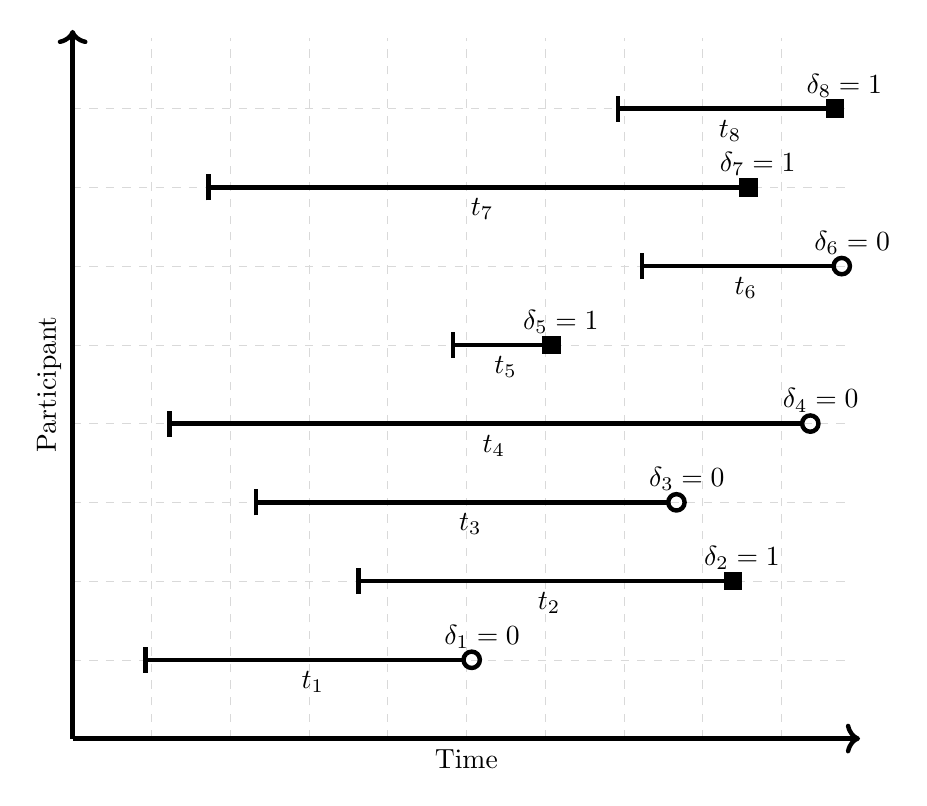
\begin{tikzpicture}[]
	\draw[help lines, color=gray!30, dashed] (9.9,0) grid (0,8.9);
	\draw[->,ultra thick] (0,0)--(10,0) node[midway, below]{Time};
	\draw[->,ultra thick] (0,0)--(0,9) node[midway, left, rotate=90, anchor=south]{Participant};
	\draw[|-{Circle[open]}, ultra thick] (0.9, 1)--(5.2,1) node[above] {$\delta_1=0$} node[below,midway] {$t_1$};
	\draw[|-{Square}, ultra thick] (3.6,2)--(8.5,2) node[above] {$\delta_2=1$} node[below, midway] {$t_2$};
	\draw[|-{Circle[open]}, ultra thick] (2.3, 3)--(7.8,3) node[above] {$\delta_3=0$} node[below,midway] {$t_3$};
	\draw[|-{Circle[open]}, ultra thick] (1.2, 4)--(9.5,4) node[above] {$\delta_4=0$} node[below, midway] {$t_4$};
	\draw[|-{Square}, ultra thick] (4.8, 5)--(6.2 ,5) node[above] {$\delta_5=1$} node[below, midway] {$t_5$};
	\draw[|-{Circle[open]}, ultra thick] (7.2, 6)--(9.9,6) node[above] {$\delta_6=0$} node[below, midway] {$t_6$};
	\draw[|-{Square}, ultra thick] (1.7, 7)--(8.7,7) node[above] {$\delta_7=1$} node[below, midway] {$t_7$};
	\draw[|-{Square}, ultra thick] (6.9, 8)--(9.8,8) node[above] {$\delta_8=1$} node[below, midway] {$t_8$};
\end{tikzpicture}
\end{document}
